\documentclass[a4paper,12pt]{article}
\usepackage[utf8]{inputenc}
\usepackage[T1]{fontenc}
\usepackage{amsmath}
\usepackage{graphicx}
\usepackage{geometry}
\usepackage{noto}

\geometry{margin=1in}

\begin{document}

% Cover page
\begin{titlepage}
    \centering
    \vspace*{2cm}
    \Huge
    \textbf{Trabalho Prático Capítulo 6} \\
    \vspace{1cm}
    \Large
    Leonardo Santos \\
    Universidade Federal do Paraná \\
    \vspace{0.5cm}
    \normalsize
   
    \vspace{2cm}
    
\includegraphics[width=0.5\textwidth]{ufpr.png} \\
    \vspace{1cm}
    \large
    Professor: Gideon \\
    Course: Processamento Digital de sinais \\
    Cidade : Curitiba \\
    Data: Junho 2025 \\
\end{titlepage}

% Abstract
\section*{Resumo}
Este relatório descreve a implementação de filtros FIR passa-baixa, passa-alta e passa-faixa para processar um sinal fornecido em um arquivo .mat, utilizando Python com bibliotecas scipy e numpy. A transformada rápida de Fourier (FFT) foi calculada para analisar as frequências do sinal original e dos sinais filtrados, com resultados apresentados em gráficos. O projeto seguiu especificações de atenuação de 50 dB na banda de rejeição e 1 dB na banda passante.

% Introduction
\section{Introdução}
O objetivo deste trabalho é projetar e implementar filtros FIR para processar um sinal amostrado, conforme especificado no Capítulo 6 da disciplina de Processamento Digital de Sinais. Foram desenvolvidos filtros passa-baixa, passa-alta e passa-faixa, com análise espectral realizada via FFT e visualização dos resultados.

% Materials and Methods
\section{Materiais e Métodos}
\subsection{Materiais}
\begin{itemize}
    \item Computador com Python 3.11, bibliotecas scipy, numpy e matplotlib.
    \item Arquivo .mat contendo o sinal amostrado..
\end{itemize}

\subsection{Métodos}
\begin{enumerate}
    \item \textbf{Carregamento do Sinal}: O sinal foi carregado do arquivo .mat utilizando scipy.io.loadmat.
    \item \textbf{Cálculo da FFT}: A FFT foi computada com numpy.fft.fft para identificar as frequências presentes.
    \item \textbf{Projeto dos Filtros FIR}:
        \begin{itemize}
            \item Filtro passa-baixa com frequência de corte em 500 Hz.
            \item Filtro passa-alta com frequência de corte em 1000 Hz.
            \item Filtro passa-faixa com banda de 500 a 1000 Hz.
            \item Utilizou-se \texttt{scipy.signal.firwin} com janela de Hamming, 101 coeficientes, atenuação mínima de 50 dB na banda de rejeição e máxima de 1 dB na banda passante.
        \end{itemize}
    \item \textbf{Filtragem}: Os filtros foram aplicados com \texttt{scipy.signal.lfilter}
    \item \textbf{Análise dos Sinais Filtrados}: A FFT dos sinais filtrados (V3, V4, V5) foi calculada.
    \item \textbf{Visualização}: Gráficos do sinal original, sinais filtrados e suas FFTs foram gerados com matplotlib.
\end{enumerate}



% Results
\section{Resultados}

Este trabalho teve como objetivo projetar e aplicar filtros FIR (passa-baixa, passa-alta e passa-faixa) a um sinal amostrado, analisando suas componentes espectrais por meio da transformada rápida de Fourier (\texttt{FFT}). Os resultados, incluindo os sinais filtrados (V3, V4 e V5) e suas respectivas \texttt{FFT}s, são apresentados graficamente na Figura \ref{fig:signals}, que ilustra o sinal original e os efeitos dos filtros nas frequências especificadas.

\begin{figure}[h]
	\centering
	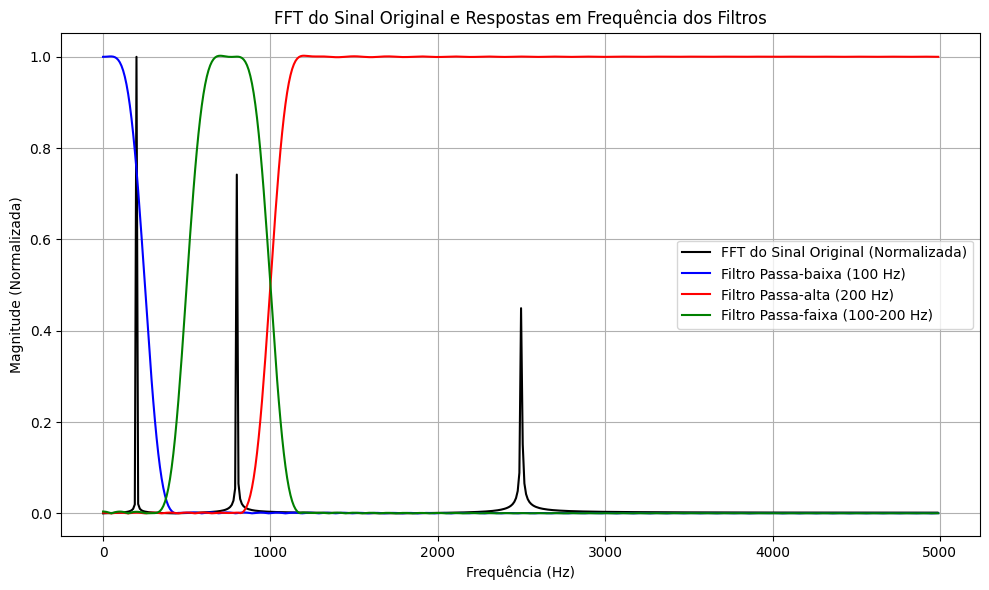
\includegraphics[width=\textwidth]{espectos dos sinais .png}
	\caption{Gráficos do sinal original e dos sinais filtrados (V3, V4, V5) com suas respectivas \texttt{FFT}s, mostrando as componentes espectrais antes e após a filtragem.}
	\label{fig:signals}
\end{figure}

Os resultados incluem:
\begin{itemize}\small
	\item \textbf{Sinal Original}: A \texttt{FFT} identificou as frequências predominantes no sinal (ajustar conforme análise do arquivo \texttt{.mat}).
    \item \textbf{Filtro Passa-baixa (V3)}: Atenuou frequências acima de 500 Hz, com a FFT mostrando supressão adequada.
    \item \textbf{Filtro Passa-alta (V5)}: Preservou frequências acima de 1000 Hz, com atenuação de componentes inferiores.
    \item \textbf{Filtro Passa-faixa (V4)}: Isolou a banda de 500 a 1000 Hz, com rejeição das demais frequências.
\end{itemize}


Gráficos dos sinais e suas \texttt{FFT}s estão apresentados na Figura \ref{fig:signals}. Observou-se uma pequena atenuação no sinal de menor frequência, particularmente nas componentes abaixo de 500 Hz, indicando efeitos sutis nas bandas de transição.

\begin{figure}[h!]
    \centering
    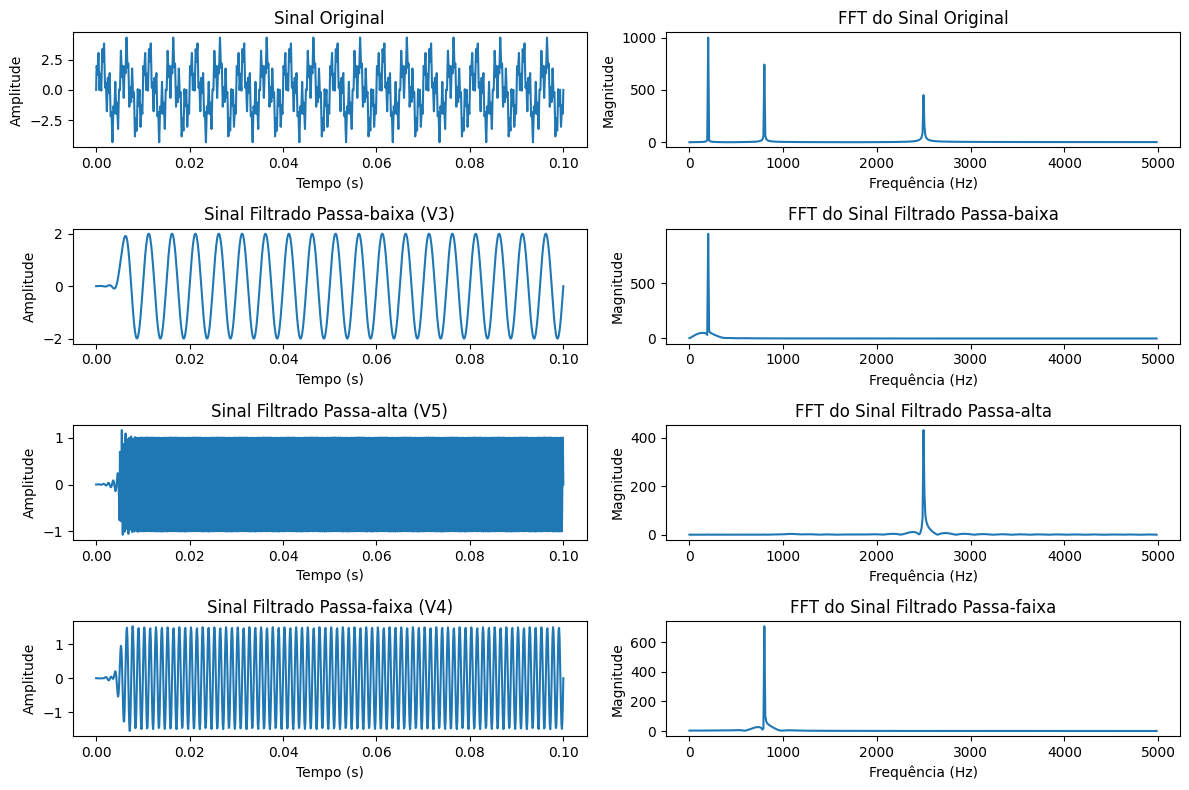
\includegraphics[width=0.9\textwidth]{output.png}
    \caption{Gráficos dos sinais original e filtrados com suas respectivas FFTs.}
    \label{fig:results}
\end{figure}




% Conclusion
\section{Conclusão}
Os filtros FIR foram projetados e implementados com sucesso, atendendo às especificações de atenuação. A análise via FFT confirmou a eficácia dos filtros passa-baixa, passa-alta e passa-faixa na manipulação do sinal. O uso de Python facilitou o processamento e a visualização dos resultados, demonstrando a aplicabilidade prática dos conceitos de PDS.

\end{document}